% Homework 17.tex 

\documentclass{article}
\usepackage{graphicx} % for figures
\usepackage{float}
\usepackage[export]{adjustbox}
\usepackage{fancyhdr}
\begin{document}

\title{Homework 11 - Physics 240\\
		Diffuse equation}
\author{Tin Tran}

\maketitle

\section{Introduction}
The goal of this homework is to apply PDE methods to solve the diffuse equation.

\section{Discussion and data}
I have modified the code to the inital and boundary conditions given in the homework and I got the following plots. I don't, however, understand why they are that way so I can't answers the question about x$_i$

\begin{figure}[H]
\centering{
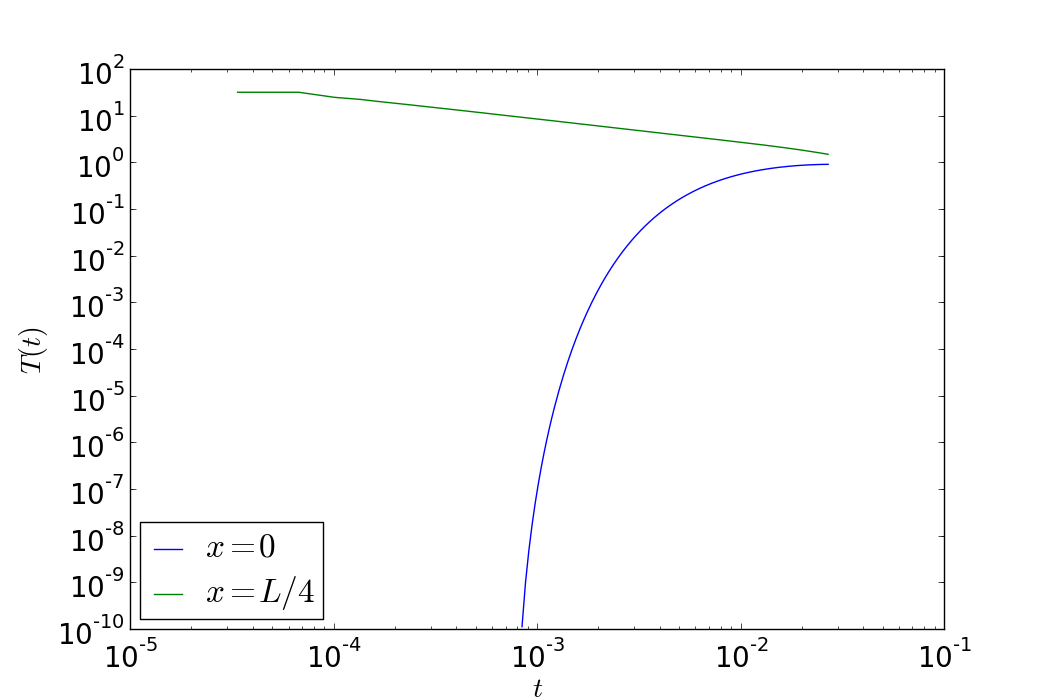
\includegraphics[max size={3 in}{4 in}]{hw17a.png}
\caption{}
}
\end{figure}

\begin{figure}[H]
\centering{
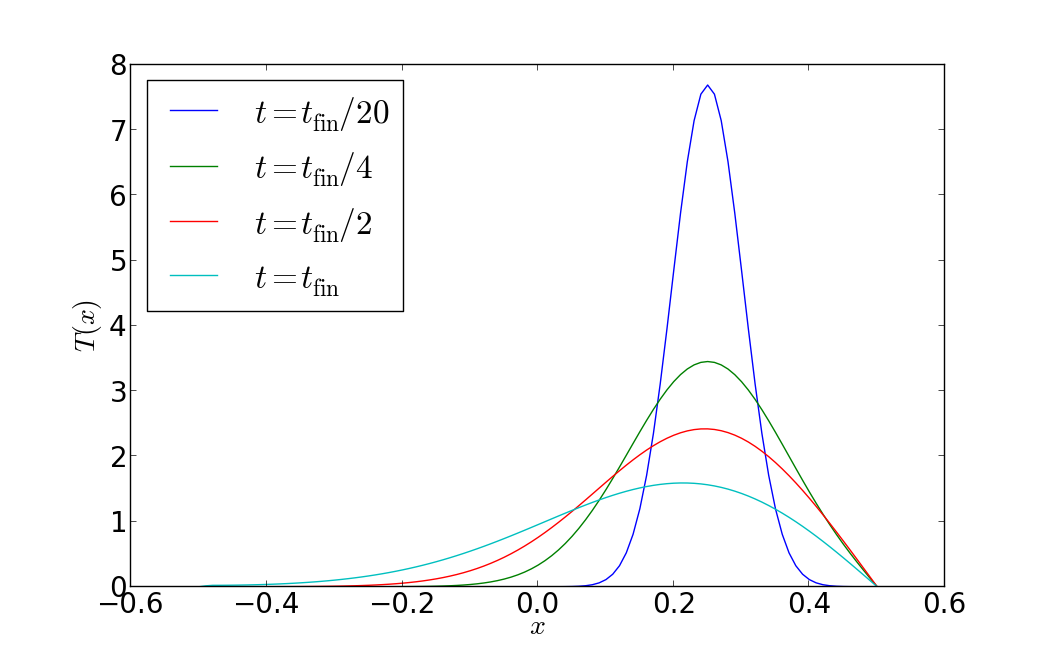
\includegraphics[max size={3 in}{4 in}]{hw17b.png}
\caption{}
}
\end{figure}

v\begin{figure}[H]
\centering{
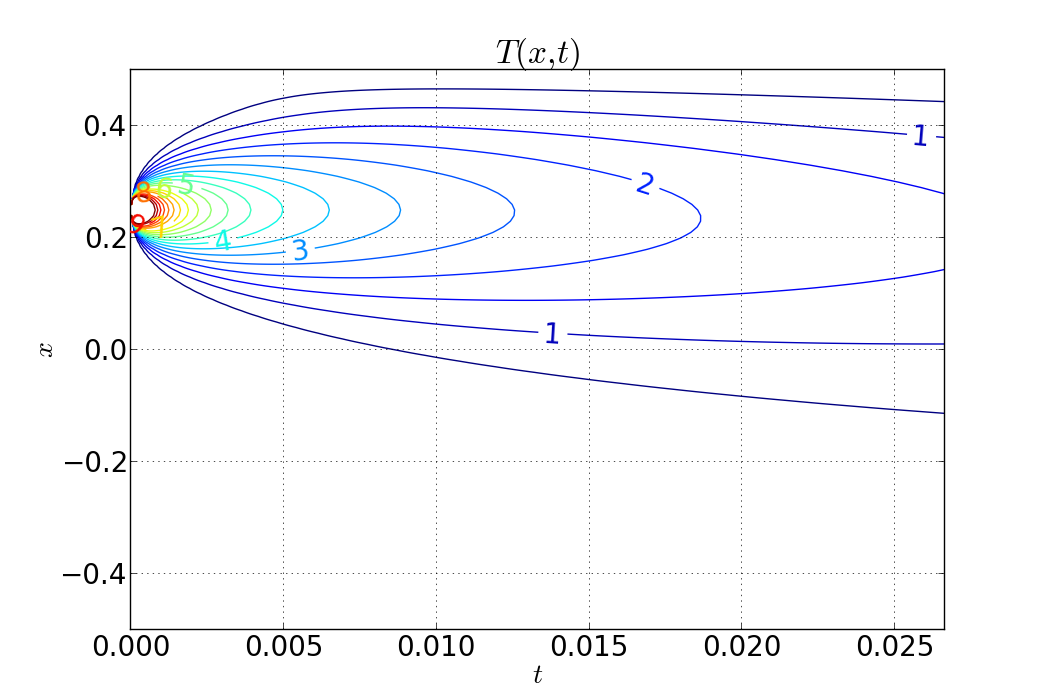
\includegraphics[max size={3 in}{4 in}]{hw17c.png}
\caption{}
}
\end{figure}


\begin{figure}[H]
\centering{
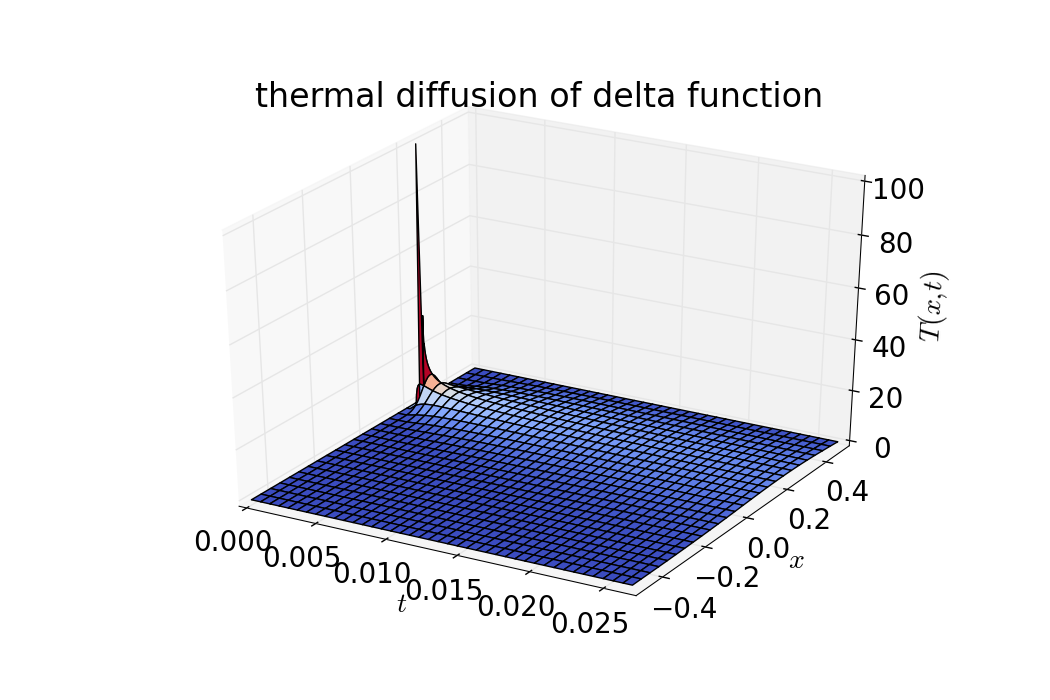
\includegraphics[max size={3 in}{4 in}]{hw17d.png}
\caption{}
}
\end{figure}



\end{document}